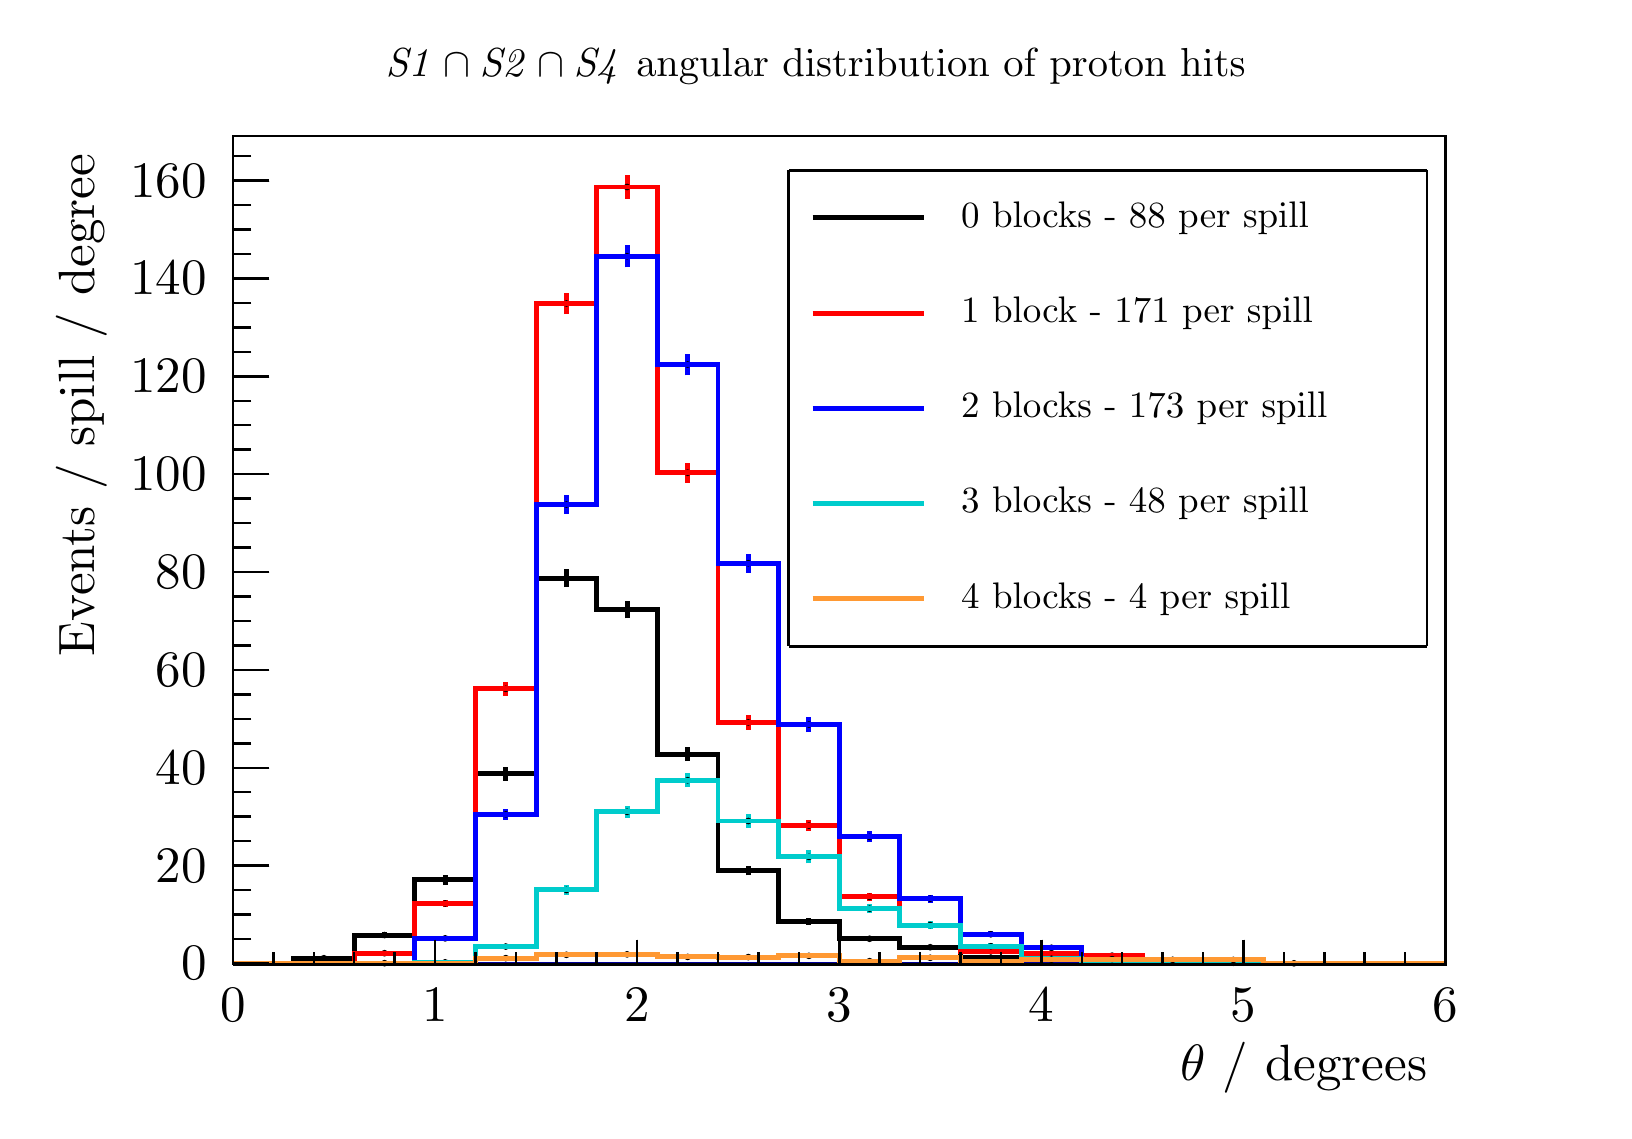
\begin{tikzpicture}
\pgfdeclareplotmark{cross} {
\pgfpathmoveto{\pgfpoint{-0.3\pgfplotmarksize}{\pgfplotmarksize}}
\pgfpathlineto{\pgfpoint{+0.3\pgfplotmarksize}{\pgfplotmarksize}}
\pgfpathlineto{\pgfpoint{+0.3\pgfplotmarksize}{0.3\pgfplotmarksize}}
\pgfpathlineto{\pgfpoint{+1\pgfplotmarksize}{0.3\pgfplotmarksize}}
\pgfpathlineto{\pgfpoint{+1\pgfplotmarksize}{-0.3\pgfplotmarksize}}
\pgfpathlineto{\pgfpoint{+0.3\pgfplotmarksize}{-0.3\pgfplotmarksize}}
\pgfpathlineto{\pgfpoint{+0.3\pgfplotmarksize}{-1.\pgfplotmarksize}}
\pgfpathlineto{\pgfpoint{-0.3\pgfplotmarksize}{-1.\pgfplotmarksize}}
\pgfpathlineto{\pgfpoint{-0.3\pgfplotmarksize}{-0.3\pgfplotmarksize}}
\pgfpathlineto{\pgfpoint{-1.\pgfplotmarksize}{-0.3\pgfplotmarksize}}
\pgfpathlineto{\pgfpoint{-1.\pgfplotmarksize}{0.3\pgfplotmarksize}}
\pgfpathlineto{\pgfpoint{-0.3\pgfplotmarksize}{0.3\pgfplotmarksize}}
\pgfpathclose
\pgfusepathqstroke
}
\pgfdeclareplotmark{cross*} {
\pgfpathmoveto{\pgfpoint{-0.3\pgfplotmarksize}{\pgfplotmarksize}}
\pgfpathlineto{\pgfpoint{+0.3\pgfplotmarksize}{\pgfplotmarksize}}
\pgfpathlineto{\pgfpoint{+0.3\pgfplotmarksize}{0.3\pgfplotmarksize}}
\pgfpathlineto{\pgfpoint{+1\pgfplotmarksize}{0.3\pgfplotmarksize}}
\pgfpathlineto{\pgfpoint{+1\pgfplotmarksize}{-0.3\pgfplotmarksize}}
\pgfpathlineto{\pgfpoint{+0.3\pgfplotmarksize}{-0.3\pgfplotmarksize}}
\pgfpathlineto{\pgfpoint{+0.3\pgfplotmarksize}{-1.\pgfplotmarksize}}
\pgfpathlineto{\pgfpoint{-0.3\pgfplotmarksize}{-1.\pgfplotmarksize}}
\pgfpathlineto{\pgfpoint{-0.3\pgfplotmarksize}{-0.3\pgfplotmarksize}}
\pgfpathlineto{\pgfpoint{-1.\pgfplotmarksize}{-0.3\pgfplotmarksize}}
\pgfpathlineto{\pgfpoint{-1.\pgfplotmarksize}{0.3\pgfplotmarksize}}
\pgfpathlineto{\pgfpoint{-0.3\pgfplotmarksize}{0.3\pgfplotmarksize}}
\pgfpathclose
\pgfusepathqfillstroke
}
\pgfdeclareplotmark{newstar} {
\pgfpathmoveto{\pgfqpoint{0pt}{\pgfplotmarksize}}
\pgfpathlineto{\pgfqpointpolar{44}{0.5\pgfplotmarksize}}
\pgfpathlineto{\pgfqpointpolar{18}{\pgfplotmarksize}}
\pgfpathlineto{\pgfqpointpolar{-20}{0.5\pgfplotmarksize}}
\pgfpathlineto{\pgfqpointpolar{-54}{\pgfplotmarksize}}
\pgfpathlineto{\pgfqpointpolar{-90}{0.5\pgfplotmarksize}}
\pgfpathlineto{\pgfqpointpolar{234}{\pgfplotmarksize}}
\pgfpathlineto{\pgfqpointpolar{198}{0.5\pgfplotmarksize}}
\pgfpathlineto{\pgfqpointpolar{162}{\pgfplotmarksize}}
\pgfpathlineto{\pgfqpointpolar{134}{0.5\pgfplotmarksize}}
\pgfpathclose
\pgfusepathqstroke
}
\pgfdeclareplotmark{newstar*} {
\pgfpathmoveto{\pgfqpoint{0pt}{\pgfplotmarksize}}
\pgfpathlineto{\pgfqpointpolar{44}{0.5\pgfplotmarksize}}
\pgfpathlineto{\pgfqpointpolar{18}{\pgfplotmarksize}}
\pgfpathlineto{\pgfqpointpolar{-20}{0.5\pgfplotmarksize}}
\pgfpathlineto{\pgfqpointpolar{-54}{\pgfplotmarksize}}
\pgfpathlineto{\pgfqpointpolar{-90}{0.5\pgfplotmarksize}}
\pgfpathlineto{\pgfqpointpolar{234}{\pgfplotmarksize}}
\pgfpathlineto{\pgfqpointpolar{198}{0.5\pgfplotmarksize}}
\pgfpathlineto{\pgfqpointpolar{162}{\pgfplotmarksize}}
\pgfpathlineto{\pgfqpointpolar{134}{0.5\pgfplotmarksize}}
\pgfpathclose
\pgfusepathqfillstroke
}
\definecolor{c}{rgb}{1,1,1};
\draw [color=c, fill=c] (0,0) rectangle (20,13.6676);
\draw [color=c, fill=c] (2.6,1.77679) rectangle (18,12.3009);
\definecolor{c}{rgb}{0,0,0};
\draw [c,line width=0.9] (2.6,1.77679) -- (2.6,12.3009) -- (18,12.3009) -- (18,1.77679) -- (2.6,1.77679);
\definecolor{c}{rgb}{1,1,1};
\draw [color=c, fill=c] (2.6,1.77679) rectangle (18,12.3009);
\definecolor{c}{rgb}{0,0,0};
\draw [c,line width=0.9] (2.6,1.77679) -- (2.6,12.3009) -- (18,12.3009) -- (18,1.77679) -- (2.6,1.77679);
\definecolor{c}{rgb}{0,0,0.6};
\draw [c,line width=0.9] (2.6,1.78961) -- (3.37,1.78961) -- (3.37,1.78961) -- (4.14,1.78961) -- (4.14,1.78961) -- (4.91,1.78961) -- (4.91,1.78961) -- (5.68,1.78961) -- (5.68,1.78961) -- (6.45,1.78961) -- (6.45,1.78961) -- (7.22,1.78961) --
 (7.22,1.78961) -- (7.99,1.78961) -- (7.99,1.78961) -- (8.76,1.78961) -- (8.76,1.78961) -- (9.53,1.78961) -- (9.53,1.78961) -- (10.3,1.78961) -- (10.3,1.78961) -- (11.07,1.78961) -- (11.07,1.78961) -- (11.84,1.78961) -- (11.84,1.78961) --
 (12.61,1.78961) -- (12.61,1.78961) -- (13.38,1.78961) -- (13.38,1.78961) -- (14.15,1.78961) -- (14.15,1.78961) -- (14.92,1.78961) -- (14.92,1.78961) -- (15.69,1.78961) -- (15.69,1.78961) -- (16.46,1.78961) -- (16.46,1.78961) -- (17.23,1.78961) --
 (17.23,1.78961) -- (18,1.78961);
\definecolor{c}{rgb}{0,0,0};
\draw [c,line width=0.9] (2.6,1.77679) -- (18,1.77679);
\draw [c,line width=0.9] (2.6,2.09251) -- (2.6,1.77679);
\draw [c,line width=0.9] (3.11333,1.93465) -- (3.11333,1.77679);
\draw [c,line width=0.9] (3.62667,1.93465) -- (3.62667,1.77679);
\draw [c,line width=0.9] (4.14,1.93465) -- (4.14,1.77679);
\draw [c,line width=0.9] (4.65333,1.93465) -- (4.65333,1.77679);
\draw [c,line width=0.9] (5.16667,2.09251) -- (5.16667,1.77679);
\draw [c,line width=0.9] (5.68,1.93465) -- (5.68,1.77679);
\draw [c,line width=0.9] (6.19333,1.93465) -- (6.19333,1.77679);
\draw [c,line width=0.9] (6.70667,1.93465) -- (6.70667,1.77679);
\draw [c,line width=0.9] (7.22,1.93465) -- (7.22,1.77679);
\draw [c,line width=0.9] (7.73333,2.09251) -- (7.73333,1.77679);
\draw [c,line width=0.9] (8.24667,1.93465) -- (8.24667,1.77679);
\draw [c,line width=0.9] (8.76,1.93465) -- (8.76,1.77679);
\draw [c,line width=0.9] (9.27333,1.93465) -- (9.27333,1.77679);
\draw [c,line width=0.9] (9.78667,1.93465) -- (9.78667,1.77679);
\draw [c,line width=0.9] (10.3,2.09251) -- (10.3,1.77679);
\draw [c,line width=0.9] (10.8133,1.93465) -- (10.8133,1.77679);
\draw [c,line width=0.9] (11.3267,1.93465) -- (11.3267,1.77679);
\draw [c,line width=0.9] (11.84,1.93465) -- (11.84,1.77679);
\draw [c,line width=0.9] (12.3533,1.93465) -- (12.3533,1.77679);
\draw [c,line width=0.9] (12.8667,2.09251) -- (12.8667,1.77679);
\draw [c,line width=0.9] (13.38,1.93465) -- (13.38,1.77679);
\draw [c,line width=0.9] (13.8933,1.93465) -- (13.8933,1.77679);
\draw [c,line width=0.9] (14.4067,1.93465) -- (14.4067,1.77679);
\draw [c,line width=0.9] (14.92,1.93465) -- (14.92,1.77679);
\draw [c,line width=0.9] (15.4333,2.09251) -- (15.4333,1.77679);
\draw [c,line width=0.9] (15.9467,1.93465) -- (15.9467,1.77679);
\draw [c,line width=0.9] (16.46,1.93465) -- (16.46,1.77679);
\draw [c,line width=0.9] (16.9733,1.93465) -- (16.9733,1.77679);
\draw [c,line width=0.9] (17.4867,1.93465) -- (17.4867,1.77679);
\draw [c,line width=0.9] (18,2.09251) -- (18,1.77679);
\draw [anchor=base] (2.6,1.05241) node[scale=1.84551, color=c, rotate=0]{0};
\draw [anchor=base] (5.16667,1.05241) node[scale=1.84551, color=c, rotate=0]{1};
\draw [anchor=base] (7.73333,1.05241) node[scale=1.84551, color=c, rotate=0]{2};
\draw [anchor=base] (10.3,1.05241) node[scale=1.84551, color=c, rotate=0]{3};
\draw [anchor=base] (12.8667,1.05241) node[scale=1.84551, color=c, rotate=0]{4};
\draw [anchor=base] (15.4333,1.05241) node[scale=1.84551, color=c, rotate=0]{5};
\draw [anchor=base] (18,1.05241) node[scale=1.84551, color=c, rotate=0]{6};
\draw [anchor= east] (18,0.464699) node[scale=1.84551, color=c, rotate=0]{$\theta$ / degrees};
\draw [c,line width=0.9] (2.6,1.77679) -- (2.6,12.3009);
\draw [c,line width=0.9] (3.062,1.78961) -- (2.6,1.78961);
\draw [c,line width=0.9] (2.831,2.10033) -- (2.6,2.10033);
\draw [c,line width=0.9] (2.831,2.41104) -- (2.6,2.41104);
\draw [c,line width=0.9] (2.831,2.72175) -- (2.6,2.72175);
\draw [c,line width=0.9] (3.062,3.03246) -- (2.6,3.03246);
\draw [c,line width=0.9] (2.831,3.34318) -- (2.6,3.34318);
\draw [c,line width=0.9] (2.831,3.65389) -- (2.6,3.65389);
\draw [c,line width=0.9] (2.831,3.9646) -- (2.6,3.9646);
\draw [c,line width=0.9] (3.062,4.27531) -- (2.6,4.27531);
\draw [c,line width=0.9] (2.831,4.58603) -- (2.6,4.58603);
\draw [c,line width=0.9] (2.831,4.89674) -- (2.6,4.89674);
\draw [c,line width=0.9] (2.831,5.20745) -- (2.6,5.20745);
\draw [c,line width=0.9] (3.062,5.51817) -- (2.6,5.51817);
\draw [c,line width=0.9] (2.831,5.82888) -- (2.6,5.82888);
\draw [c,line width=0.9] (2.831,6.13959) -- (2.6,6.13959);
\draw [c,line width=0.9] (2.831,6.4503) -- (2.6,6.4503);
\draw [c,line width=0.9] (3.062,6.76102) -- (2.6,6.76102);
\draw [c,line width=0.9] (2.831,7.07173) -- (2.6,7.07173);
\draw [c,line width=0.9] (2.831,7.38244) -- (2.6,7.38244);
\draw [c,line width=0.9] (2.831,7.69315) -- (2.6,7.69315);
\draw [c,line width=0.9] (3.062,8.00387) -- (2.6,8.00387);
\draw [c,line width=0.9] (2.831,8.31458) -- (2.6,8.31458);
\draw [c,line width=0.9] (2.831,8.62529) -- (2.6,8.62529);
\draw [c,line width=0.9] (2.831,8.93601) -- (2.6,8.93601);
\draw [c,line width=0.9] (3.062,9.24672) -- (2.6,9.24672);
\draw [c,line width=0.9] (2.831,9.55743) -- (2.6,9.55743);
\draw [c,line width=0.9] (2.831,9.86814) -- (2.6,9.86814);
\draw [c,line width=0.9] (2.831,10.1789) -- (2.6,10.1789);
\draw [c,line width=0.9] (3.062,10.4896) -- (2.6,10.4896);
\draw [c,line width=0.9] (2.831,10.8003) -- (2.6,10.8003);
\draw [c,line width=0.9] (2.831,11.111) -- (2.6,11.111);
\draw [c,line width=0.9] (2.831,11.4217) -- (2.6,11.4217);
\draw [c,line width=0.9] (3.062,11.7324) -- (2.6,11.7324);
\draw [c,line width=0.9] (3.062,1.78961) -- (2.6,1.78961);
\draw [c,line width=0.9] (3.062,11.7324) -- (2.6,11.7324);
\draw [c,line width=0.9] (2.831,12.0431) -- (2.6,12.0431);
\draw [anchor= east] (2.5,1.78961) node[scale=1.84551, color=c, rotate=0]{0};
\draw [anchor= east] (2.5,3.03246) node[scale=1.84551, color=c, rotate=0]{20};
\draw [anchor= east] (2.5,4.27531) node[scale=1.84551, color=c, rotate=0]{40};
\draw [anchor= east] (2.5,5.51817) node[scale=1.84551, color=c, rotate=0]{60};
\draw [anchor= east] (2.5,6.76102) node[scale=1.84551, color=c, rotate=0]{80};
\draw [anchor= east] (2.5,8.00387) node[scale=1.84551, color=c, rotate=0]{100};
\draw [anchor= east] (2.5,9.24672) node[scale=1.84551, color=c, rotate=0]{120};
\draw [anchor= east] (2.5,10.4896) node[scale=1.84551, color=c, rotate=0]{140};
\draw [anchor= east] (2.5,11.7324) node[scale=1.84551, color=c, rotate=0]{160};
\draw [anchor= east] (0.68,12.3009) node[scale=1.84551, color=c, rotate=90]{Events / spill / degree};
\draw [c,line width=1.8] (3.755,1.83612) -- (3.755,1.85682);
\draw [c,line width=1.8] (3.755,1.85682) -- (3.755,1.87752);
\foreach \P in {(3.755,1.85682)}{\draw[mark options={color=c,fill=c},mark size=2.402402pt,mark=*,mark size=1pt] plot coordinates {\P};}
\draw [c,line width=1.8] (4.525,2.10757) -- (4.525,2.1504);
\draw [c,line width=1.8] (4.525,2.1504) -- (4.525,2.19323);
\foreach \P in {(4.525,2.1504)}{\draw[mark options={color=c,fill=c},mark size=2.402402pt,mark=*,mark size=1pt] plot coordinates {\P};}
\draw [c,line width=1.8] (5.295,2.78525) -- (5.295,2.85216);
\draw [c,line width=1.8] (5.295,2.85216) -- (5.295,2.91907);
\foreach \P in {(5.295,2.85216)}{\draw[mark options={color=c,fill=c},mark size=2.402402pt,mark=*,mark size=1pt] plot coordinates {\P};}
\draw [c,line width=1.8] (6.065,4.11205) -- (6.065,4.20174);
\draw [c,line width=1.8] (6.065,4.20174) -- (6.065,4.29142);
\foreach \P in {(6.065,4.20174)}{\draw[mark options={color=c,fill=c},mark size=2.402402pt,mark=*,mark size=1pt] plot coordinates {\P};}
\draw [c,line width=1.8] (6.835,6.56912) -- (6.835,6.68379);
\draw [c,line width=1.8] (6.835,6.68379) -- (6.835,6.79847);
\foreach \P in {(6.835,6.68379)}{\draw[mark options={color=c,fill=c},mark size=2.402402pt,mark=*,mark size=1pt] plot coordinates {\P};}
\draw [c,line width=1.8] (7.605,6.17333) -- (7.605,6.28243);
\draw [c,line width=1.8] (7.605,6.28243) -- (7.605,6.39154);
\foreach \P in {(7.605,6.28243)}{\draw[mark options={color=c,fill=c},mark size=2.402402pt,mark=*,mark size=1pt] plot coordinates {\P};}
\draw [c,line width=1.8] (8.375,4.36076) -- (8.375,4.44822);
\draw [c,line width=1.8] (8.375,4.44822) -- (8.375,4.53567);
\foreach \P in {(8.375,4.44822)}{\draw[mark options={color=c,fill=c},mark size=2.402402pt,mark=*,mark size=1pt] plot coordinates {\P};}
\draw [c,line width=1.8] (9.145,2.9086) -- (9.145,2.96867);
\draw [c,line width=1.8] (9.145,2.96867) -- (9.145,3.02874);
\foreach \P in {(9.145,2.96867)}{\draw[mark options={color=c,fill=c},mark size=2.402402pt,mark=*,mark size=1pt] plot coordinates {\P};}
\draw [c,line width=1.8] (9.915,2.28161) -- (9.915,2.32261);
\draw [c,line width=1.8] (9.915,2.32261) -- (9.915,2.36361);
\foreach \P in {(9.915,2.32261)}{\draw[mark options={color=c,fill=c},mark size=2.402402pt,mark=*,mark size=1pt] plot coordinates {\P};}
\draw [c,line width=1.8] (10.685,2.07185) -- (10.685,2.10415);
\draw [c,line width=1.8] (10.685,2.10415) -- (10.685,2.13644);
\foreach \P in {(10.685,2.10415)}{\draw[mark options={color=c,fill=c},mark size=2.402402pt,mark=*,mark size=1pt] plot coordinates {\P};}
\draw [c,line width=1.8] (11.455,1.97057) -- (11.455,1.9963);
\draw [c,line width=1.8] (11.455,1.9963) -- (11.455,2.02203);
\foreach \P in {(11.455,1.9963)}{\draw[mark options={color=c,fill=c},mark size=2.402402pt,mark=*,mark size=1pt] plot coordinates {\P};}
\draw [c,line width=1.8] (12.225,1.84644) -- (12.225,1.86292);
\draw [c,line width=1.8] (12.225,1.86292) -- (12.225,1.87941);
\foreach \P in {(12.225,1.86292)}{\draw[mark options={color=c,fill=c},mark size=2.402402pt,mark=*,mark size=1pt] plot coordinates {\P};}
\draw [c,line width=1.8] (12.995,1.82858) -- (12.995,1.84327);
\draw [c,line width=1.8] (12.995,1.84327) -- (12.995,1.85797);
\foreach \P in {(12.995,1.84327)}{\draw[mark options={color=c,fill=c},mark size=2.402402pt,mark=*,mark size=1pt] plot coordinates {\P};}
\draw [c,line width=1.8] (13.765,1.79714) -- (13.765,1.80802);
\draw [c,line width=1.8] (13.765,1.80802) -- (13.765,1.81891);
\foreach \P in {(13.765,1.80802)}{\draw[mark options={color=c,fill=c},mark size=2.402402pt,mark=*,mark size=1pt] plot coordinates {\P};}
\draw [c,line width=1.8] (14.535,1.80395) -- (14.535,1.81716);
\draw [c,line width=1.8] (14.535,1.81716) -- (14.535,1.83037);
\foreach \P in {(14.535,1.81716)}{\draw[mark options={color=c,fill=c},mark size=2.402402pt,mark=*,mark size=1pt] plot coordinates {\P};}
\draw [c,line width=1.8] (16.075,1.78303) -- (16.075,1.79187);
\draw [c,line width=1.8] (16.075,1.79187) -- (16.075,1.80072);
\foreach \P in {(16.075,1.79187)}{\draw[mark options={color=c,fill=c},mark size=2.402402pt,mark=*,mark size=1pt] plot coordinates {\P};}
\draw [c,line width=1.8] (2.6,1.78961) -- (3.37,1.78961) -- (3.37,1.85682) -- (4.14,1.85682) -- (4.14,2.1504) -- (4.91,2.1504) -- (4.91,2.85216) -- (5.68,2.85216) -- (5.68,4.20174) -- (6.45,4.20174) -- (6.45,6.68379) -- (7.22,6.68379) --
 (7.22,6.28243) -- (7.99,6.28243) -- (7.99,4.44822) -- (8.76,4.44822) -- (8.76,2.96867) -- (9.53,2.96867) -- (9.53,2.32261) -- (10.3,2.32261) -- (10.3,2.10415) -- (11.07,2.10415) -- (11.07,1.9963) -- (11.84,1.9963) -- (11.84,1.86292) --
 (12.61,1.86292) -- (12.61,1.84327) -- (13.38,1.84327) -- (13.38,1.80802) -- (14.15,1.80802) -- (14.15,1.81716) -- (14.92,1.81716) -- (14.92,1.78961) -- (15.69,1.78961) -- (15.69,1.79187) -- (16.46,1.79187) -- (16.46,1.78961) -- (17.23,1.78961) --
 (17.23,1.78961) -- (18,1.78961);
\definecolor{c}{rgb}{1,0,0};
\draw [c,line width=1.8] (4.525,1.89801) -- (4.525,1.9203);
\draw [c,line width=1.8] (4.525,1.9203) -- (4.525,1.94259);
\definecolor{c}{rgb}{0,0,0};
\foreach \P in {(4.525,1.9203)}{\draw[mark options={color=c,fill=c},mark size=2.402402pt,mark=*,mark size=1pt] plot coordinates {\P};}
\definecolor{c}{rgb}{1,0,0};
\draw [c,line width=1.8] (5.295,2.50701) -- (5.295,2.55253);
\draw [c,line width=1.8] (5.295,2.55253) -- (5.295,2.59805);
\definecolor{c}{rgb}{0,0,0};
\foreach \P in {(5.295,2.55253)}{\draw[mark options={color=c,fill=c},mark size=2.402402pt,mark=*,mark size=1pt] plot coordinates {\P};}
\definecolor{c}{rgb}{1,0,0};
\draw [c,line width=1.8] (6.065,5.18525) -- (6.065,5.27744);
\draw [c,line width=1.8] (6.065,5.27744) -- (6.065,5.36964);
\definecolor{c}{rgb}{0,0,0};
\foreach \P in {(6.065,5.27744)}{\draw[mark options={color=c,fill=c},mark size=2.402402pt,mark=*,mark size=1pt] plot coordinates {\P};}
\definecolor{c}{rgb}{1,0,0};
\draw [c,line width=1.8] (6.835,10.0365) -- (6.835,10.1718);
\draw [c,line width=1.8] (6.835,10.1718) -- (6.835,10.307);
\definecolor{c}{rgb}{0,0,0};
\foreach \P in {(6.835,10.1718)}{\draw[mark options={color=c,fill=c},mark size=2.402402pt,mark=*,mark size=1pt] plot coordinates {\P};}
\definecolor{c}{rgb}{1,0,0};
\draw [c,line width=1.8] (7.605,11.5018) -- (7.605,11.6511);
\draw [c,line width=1.8] (7.605,11.6511) -- (7.605,11.8003);
\definecolor{c}{rgb}{0,0,0};
\foreach \P in {(7.605,11.6511)}{\draw[mark options={color=c,fill=c},mark size=2.402402pt,mark=*,mark size=1pt] plot coordinates {\P};}
\definecolor{c}{rgb}{1,0,0};
\draw [c,line width=1.8] (8.375,7.89387) -- (8.375,8.02249);
\draw [c,line width=1.8] (8.375,8.02249) -- (8.375,8.15111);
\definecolor{c}{rgb}{0,0,0};
\foreach \P in {(8.375,8.02249)}{\draw[mark options={color=c,fill=c},mark size=2.402402pt,mark=*,mark size=1pt] plot coordinates {\P};}
\definecolor{c}{rgb}{1,0,0};
\draw [c,line width=1.8] (9.145,4.75881) -- (9.145,4.85158);
\draw [c,line width=1.8] (9.145,4.85158) -- (9.145,4.94436);
\definecolor{c}{rgb}{0,0,0};
\foreach \P in {(9.145,4.85158)}{\draw[mark options={color=c,fill=c},mark size=2.402402pt,mark=*,mark size=1pt] plot coordinates {\P};}
\definecolor{c}{rgb}{1,0,0};
\draw [c,line width=1.8] (9.915,3.46923) -- (9.915,3.54067);
\draw [c,line width=1.8] (9.915,3.54067) -- (9.915,3.6121);
\definecolor{c}{rgb}{0,0,0};
\foreach \P in {(9.915,3.54067)}{\draw[mark options={color=c,fill=c},mark size=2.402402pt,mark=*,mark size=1pt] plot coordinates {\P};}
\definecolor{c}{rgb}{1,0,0};
\draw [c,line width=1.8] (10.685,2.585) -- (10.685,2.63568);
\draw [c,line width=1.8] (10.685,2.63568) -- (10.685,2.68635);
\definecolor{c}{rgb}{0,0,0};
\foreach \P in {(10.685,2.63568)}{\draw[mark options={color=c,fill=c},mark size=2.402402pt,mark=*,mark size=1pt] plot coordinates {\P};}
\definecolor{c}{rgb}{1,0,0};
\draw [c,line width=1.8] (11.455,2.23259) -- (11.455,2.27254);
\draw [c,line width=1.8] (11.455,2.27254) -- (11.455,2.31249);
\definecolor{c}{rgb}{0,0,0};
\foreach \P in {(11.455,2.27254)}{\draw[mark options={color=c,fill=c},mark size=2.402402pt,mark=*,mark size=1pt] plot coordinates {\P};}
\definecolor{c}{rgb}{1,0,0};
\draw [c,line width=1.8] (12.225,1.92368) -- (12.225,1.9462);
\draw [c,line width=1.8] (12.225,1.9462) -- (12.225,1.96872);
\definecolor{c}{rgb}{0,0,0};
\foreach \P in {(12.225,1.9462)}{\draw[mark options={color=c,fill=c},mark size=2.402402pt,mark=*,mark size=1pt] plot coordinates {\P};}
\definecolor{c}{rgb}{1,0,0};
\draw [c,line width=1.8] (12.995,1.89628) -- (12.995,1.91749);
\draw [c,line width=1.8] (12.995,1.91749) -- (12.995,1.9387);
\definecolor{c}{rgb}{0,0,0};
\foreach \P in {(12.995,1.91749)}{\draw[mark options={color=c,fill=c},mark size=2.402402pt,mark=*,mark size=1pt] plot coordinates {\P};}
\definecolor{c}{rgb}{1,0,0};
\draw [c,line width=1.8] (13.765,1.86905) -- (13.765,1.88935);
\draw [c,line width=1.8] (13.765,1.88935) -- (13.765,1.90964);
\definecolor{c}{rgb}{0,0,0};
\foreach \P in {(13.765,1.88935)}{\draw[mark options={color=c,fill=c},mark size=2.402402pt,mark=*,mark size=1pt] plot coordinates {\P};}
\definecolor{c}{rgb}{1,0,0};
\draw [c,line width=1.8] (14.535,1.80747) -- (14.535,1.82111);
\draw [c,line width=1.8] (14.535,1.82111) -- (14.535,1.83475);
\definecolor{c}{rgb}{0,0,0};
\foreach \P in {(14.535,1.82111)}{\draw[mark options={color=c,fill=c},mark size=2.402402pt,mark=*,mark size=1pt] plot coordinates {\P};}
\definecolor{c}{rgb}{1,0,0};
\draw [c,line width=1.8] (15.305,1.7851) -- (15.305,1.79892);
\draw [c,line width=1.8] (15.305,1.79892) -- (15.305,1.81273);
\definecolor{c}{rgb}{0,0,0};
\foreach \P in {(15.305,1.79892)}{\draw[mark options={color=c,fill=c},mark size=2.402402pt,mark=*,mark size=1pt] plot coordinates {\P};}
\definecolor{c}{rgb}{1,0,0};
\draw [c,line width=1.8] (2.6,1.78961) -- (3.37,1.78961) -- (3.37,1.78961) -- (4.14,1.78961) -- (4.14,1.9203) -- (4.91,1.9203) -- (4.91,2.55253) -- (5.68,2.55253) -- (5.68,5.27744) -- (6.45,5.27744) -- (6.45,10.1718) -- (7.22,10.1718) --
 (7.22,11.6511) -- (7.99,11.6511) -- (7.99,8.02249) -- (8.76,8.02249) -- (8.76,4.85158) -- (9.53,4.85158) -- (9.53,3.54067) -- (10.3,3.54067) -- (10.3,2.63568) -- (11.07,2.63568) -- (11.07,2.27254) -- (11.84,2.27254) -- (11.84,1.9462) --
 (12.61,1.9462) -- (12.61,1.91749) -- (13.38,1.91749) -- (13.38,1.88935) -- (14.15,1.88935) -- (14.15,1.82111) -- (14.92,1.82111) -- (14.92,1.79892) -- (15.69,1.79892) -- (15.69,1.78961) -- (16.46,1.78961) -- (16.46,1.78961) -- (17.23,1.78961) --
 (17.23,1.78961) -- (18,1.78961);
\definecolor{c}{rgb}{0,0,1};
\draw [c,line width=1.8] (4.525,1.77679) -- (4.525,1.79359);
\draw [c,line width=1.8] (4.525,1.79359) -- (4.525,1.81039);
\definecolor{c}{rgb}{0,0,0};
\foreach \P in {(4.525,1.79359)}{\draw[mark options={color=c,fill=c},mark size=2.402402pt,mark=*,mark size=1pt] plot coordinates {\P};}
\definecolor{c}{rgb}{0,0,1};
\draw [c,line width=1.8] (5.295,2.07588) -- (5.295,2.10909);
\draw [c,line width=1.8] (5.295,2.10909) -- (5.295,2.14229);
\definecolor{c}{rgb}{0,0,0};
\foreach \P in {(5.295,2.10909)}{\draw[mark options={color=c,fill=c},mark size=2.402402pt,mark=*,mark size=1pt] plot coordinates {\P};}
\definecolor{c}{rgb}{0,0,1};
\draw [c,line width=1.8] (6.065,3.61234) -- (6.065,3.68387);
\draw [c,line width=1.8] (6.065,3.68387) -- (6.065,3.75539);
\definecolor{c}{rgb}{0,0,0};
\foreach \P in {(6.065,3.68387)}{\draw[mark options={color=c,fill=c},mark size=2.402402pt,mark=*,mark size=1pt] plot coordinates {\P};}
\definecolor{c}{rgb}{0,0,1};
\draw [c,line width=1.8] (6.835,7.49994) -- (6.835,7.61834);
\draw [c,line width=1.8] (6.835,7.61834) -- (6.835,7.73675);
\definecolor{c}{rgb}{0,0,0};
\foreach \P in {(6.835,7.61834)}{\draw[mark options={color=c,fill=c},mark size=2.402402pt,mark=*,mark size=1pt] plot coordinates {\P};}
\definecolor{c}{rgb}{0,0,1};
\draw [c,line width=1.8] (7.605,10.6294) -- (7.605,10.7718);
\draw [c,line width=1.8] (7.605,10.7718) -- (7.605,10.9143);
\definecolor{c}{rgb}{0,0,0};
\foreach \P in {(7.605,10.7718)}{\draw[mark options={color=c,fill=c},mark size=2.402402pt,mark=*,mark size=1pt] plot coordinates {\P};}
\definecolor{c}{rgb}{0,0,1};
\draw [c,line width=1.8] (8.375,9.25722) -- (8.375,9.39648);
\draw [c,line width=1.8] (8.375,9.39648) -- (8.375,9.53574);
\definecolor{c}{rgb}{0,0,0};
\foreach \P in {(8.375,9.39648)}{\draw[mark options={color=c,fill=c},mark size=2.402402pt,mark=*,mark size=1pt] plot coordinates {\P};}
\definecolor{c}{rgb}{0,0,1};
\draw [c,line width=1.8] (9.145,6.74966) -- (9.145,6.87308);
\draw [c,line width=1.8] (9.145,6.87308) -- (9.145,6.9965);
\definecolor{c}{rgb}{0,0,0};
\foreach \P in {(9.145,6.87308)}{\draw[mark options={color=c,fill=c},mark size=2.402402pt,mark=*,mark size=1pt] plot coordinates {\P};}
\definecolor{c}{rgb}{0,0,1};
\draw [c,line width=1.8] (9.915,4.72725) -- (9.915,4.82417);
\draw [c,line width=1.8] (9.915,4.82417) -- (9.915,4.92109);
\definecolor{c}{rgb}{0,0,0};
\foreach \P in {(9.915,4.82417)}{\draw[mark options={color=c,fill=c},mark size=2.402402pt,mark=*,mark size=1pt] plot coordinates {\P};}
\definecolor{c}{rgb}{0,0,1};
\draw [c,line width=1.8] (10.685,3.32653) -- (10.685,3.39658);
\draw [c,line width=1.8] (10.685,3.39658) -- (10.685,3.46664);
\definecolor{c}{rgb}{0,0,0};
\foreach \P in {(10.685,3.39658)}{\draw[mark options={color=c,fill=c},mark size=2.402402pt,mark=*,mark size=1pt] plot coordinates {\P};}
\definecolor{c}{rgb}{0,0,1};
\draw [c,line width=1.8] (11.455,2.56088) -- (11.455,2.6127);
\draw [c,line width=1.8] (11.455,2.6127) -- (11.455,2.66452);
\definecolor{c}{rgb}{0,0,0};
\foreach \P in {(11.455,2.6127)}{\draw[mark options={color=c,fill=c},mark size=2.402402pt,mark=*,mark size=1pt] plot coordinates {\P};}
\definecolor{c}{rgb}{0,0,1};
\draw [c,line width=1.8] (12.225,2.1243) -- (12.225,2.16065);
\draw [c,line width=1.8] (12.225,2.16065) -- (12.225,2.19701);
\definecolor{c}{rgb}{0,0,0};
\foreach \P in {(12.225,2.16065)}{\draw[mark options={color=c,fill=c},mark size=2.402402pt,mark=*,mark size=1pt] plot coordinates {\P};}
\definecolor{c}{rgb}{0,0,1};
\draw [c,line width=1.8] (12.995,1.96234) -- (12.995,1.98963);
\draw [c,line width=1.8] (12.995,1.98963) -- (12.995,2.01691);
\definecolor{c}{rgb}{0,0,0};
\foreach \P in {(12.995,1.98963)}{\draw[mark options={color=c,fill=c},mark size=2.402402pt,mark=*,mark size=1pt] plot coordinates {\P};}
\definecolor{c}{rgb}{0,0,1};
\draw [c,line width=1.8] (13.765,1.81803) -- (13.765,1.83692);
\draw [c,line width=1.8] (13.765,1.83692) -- (13.765,1.8558);
\definecolor{c}{rgb}{0,0,0};
\foreach \P in {(13.765,1.83692)}{\draw[mark options={color=c,fill=c},mark size=2.402402pt,mark=*,mark size=1pt] plot coordinates {\P};}
\definecolor{c}{rgb}{0,0,1};
\draw [c,line width=1.8] (14.535,1.80853) -- (14.535,1.8281);
\draw [c,line width=1.8] (14.535,1.8281) -- (14.535,1.84767);
\definecolor{c}{rgb}{0,0,0};
\foreach \P in {(14.535,1.8281)}{\draw[mark options={color=c,fill=c},mark size=2.402402pt,mark=*,mark size=1pt] plot coordinates {\P};}
\definecolor{c}{rgb}{0,0,1};
\draw [c,line width=1.8] (2.6,1.78961) -- (3.37,1.78961) -- (3.37,1.78961) -- (4.14,1.78961) -- (4.14,1.79359) -- (4.91,1.79359) -- (4.91,2.10909) -- (5.68,2.10909) -- (5.68,3.68387) -- (6.45,3.68387) -- (6.45,7.61834) -- (7.22,7.61834) --
 (7.22,10.7718) -- (7.99,10.7718) -- (7.99,9.39648) -- (8.76,9.39648) -- (8.76,6.87308) -- (9.53,6.87308) -- (9.53,4.82417) -- (10.3,4.82417) -- (10.3,3.39658) -- (11.07,3.39658) -- (11.07,2.6127) -- (11.84,2.6127) -- (11.84,2.16065) --
 (12.61,2.16065) -- (12.61,1.98963) -- (13.38,1.98963) -- (13.38,1.83692) -- (14.15,1.83692) -- (14.15,1.8281) -- (14.92,1.8281) -- (14.92,1.78961) -- (15.69,1.78961) -- (15.69,1.78961) -- (16.46,1.78961) -- (16.46,1.78961) -- (17.23,1.78961) --
 (17.23,1.78961) -- (18,1.78961);
\definecolor{c}{rgb}{0,0.8,0.8};
\draw [c,line width=1.8] (5.295,1.78639) -- (5.295,1.80434);
\draw [c,line width=1.8] (5.295,1.80434) -- (5.295,1.82228);
\definecolor{c}{rgb}{0,0,0};
\foreach \P in {(5.295,1.80434)}{\draw[mark options={color=c,fill=c},mark size=2.402402pt,mark=*,mark size=1pt] plot coordinates {\P};}
\definecolor{c}{rgb}{0,0.8,0.8};
\draw [c,line width=1.8] (6.065,1.97366) -- (6.065,2.00511);
\draw [c,line width=1.8] (6.065,2.00511) -- (6.065,2.03656);
\definecolor{c}{rgb}{0,0,0};
\foreach \P in {(6.065,2.00511)}{\draw[mark options={color=c,fill=c},mark size=2.402402pt,mark=*,mark size=1pt] plot coordinates {\P};}
\definecolor{c}{rgb}{0,0.8,0.8};
\draw [c,line width=1.8] (6.835,2.66454) -- (6.835,2.72346);
\draw [c,line width=1.8] (6.835,2.72346) -- (6.835,2.78238);
\definecolor{c}{rgb}{0,0,0};
\foreach \P in {(6.835,2.72346)}{\draw[mark options={color=c,fill=c},mark size=2.402402pt,mark=*,mark size=1pt] plot coordinates {\P};}
\definecolor{c}{rgb}{0,0.8,0.8};
\draw [c,line width=1.8] (7.605,3.63856) -- (7.605,3.71585);
\draw [c,line width=1.8] (7.605,3.71585) -- (7.605,3.79313);
\definecolor{c}{rgb}{0,0,0};
\foreach \P in {(7.605,3.71585)}{\draw[mark options={color=c,fill=c},mark size=2.402402pt,mark=*,mark size=1pt] plot coordinates {\P};}
\definecolor{c}{rgb}{0,0.8,0.8};
\draw [c,line width=1.8] (8.375,4.02845) -- (8.375,4.11678);
\draw [c,line width=1.8] (8.375,4.11678) -- (8.375,4.2051);
\definecolor{c}{rgb}{0,0,0};
\foreach \P in {(8.375,4.11678)}{\draw[mark options={color=c,fill=c},mark size=2.402402pt,mark=*,mark size=1pt] plot coordinates {\P};}
\definecolor{c}{rgb}{0,0.8,0.8};
\draw [c,line width=1.8] (9.145,3.51018) -- (9.145,3.59936);
\draw [c,line width=1.8] (9.145,3.59936) -- (9.145,3.68853);
\definecolor{c}{rgb}{0,0,0};
\foreach \P in {(9.145,3.59936)}{\draw[mark options={color=c,fill=c},mark size=2.402402pt,mark=*,mark size=1pt] plot coordinates {\P};}
\definecolor{c}{rgb}{0,0.8,0.8};
\draw [c,line width=1.8] (9.915,3.06138) -- (9.915,3.14364);
\draw [c,line width=1.8] (9.915,3.14364) -- (9.915,3.22591);
\definecolor{c}{rgb}{0,0,0};
\foreach \P in {(9.915,3.14364)}{\draw[mark options={color=c,fill=c},mark size=2.402402pt,mark=*,mark size=1pt] plot coordinates {\P};}
\definecolor{c}{rgb}{0,0.8,0.8};
\draw [c,line width=1.8] (10.685,2.42885) -- (10.685,2.48534);
\draw [c,line width=1.8] (10.685,2.48534) -- (10.685,2.54183);
\definecolor{c}{rgb}{0,0,0};
\foreach \P in {(10.685,2.48534)}{\draw[mark options={color=c,fill=c},mark size=2.402402pt,mark=*,mark size=1pt] plot coordinates {\P};}
\definecolor{c}{rgb}{0,0.8,0.8};
\draw [c,line width=1.8] (11.455,2.22851) -- (11.455,2.27834);
\draw [c,line width=1.8] (11.455,2.27834) -- (11.455,2.32817);
\definecolor{c}{rgb}{0,0,0};
\foreach \P in {(11.455,2.27834)}{\draw[mark options={color=c,fill=c},mark size=2.402402pt,mark=*,mark size=1pt] plot coordinates {\P};}
\definecolor{c}{rgb}{0,0.8,0.8};
\draw [c,line width=1.8] (12.225,1.97192) -- (12.225,2.00894);
\draw [c,line width=1.8] (12.225,2.00894) -- (12.225,2.04596);
\definecolor{c}{rgb}{0,0,0};
\foreach \P in {(12.225,2.00894)}{\draw[mark options={color=c,fill=c},mark size=2.402402pt,mark=*,mark size=1pt] plot coordinates {\P};}
\definecolor{c}{rgb}{0,0.8,0.8};
\draw [c,line width=1.8] (12.995,1.8258) -- (12.995,1.84994);
\draw [c,line width=1.8] (12.995,1.84994) -- (12.995,1.87409);
\definecolor{c}{rgb}{0,0,0};
\foreach \P in {(12.995,1.84994)}{\draw[mark options={color=c,fill=c},mark size=2.402402pt,mark=*,mark size=1pt] plot coordinates {\P};}
\definecolor{c}{rgb}{0,0.8,0.8};
\draw [c,line width=1.8] (14.535,1.79439) -- (14.535,1.81652);
\draw [c,line width=1.8] (14.535,1.81652) -- (14.535,1.83864);
\definecolor{c}{rgb}{0,0,0};
\foreach \P in {(14.535,1.81652)}{\draw[mark options={color=c,fill=c},mark size=2.402402pt,mark=*,mark size=1pt] plot coordinates {\P};}
\definecolor{c}{rgb}{0,0.8,0.8};
\draw [c,line width=1.8] (2.6,1.78961) -- (3.37,1.78961) -- (3.37,1.78961) -- (4.14,1.78961) -- (4.14,1.78961) -- (4.91,1.78961) -- (4.91,1.80434) -- (5.68,1.80434) -- (5.68,2.00511) -- (6.45,2.00511) -- (6.45,2.72346) -- (7.22,2.72346) --
 (7.22,3.71585) -- (7.99,3.71585) -- (7.99,4.11678) -- (8.76,4.11678) -- (8.76,3.59936) -- (9.53,3.59936) -- (9.53,3.14364) -- (10.3,3.14364) -- (10.3,2.48534) -- (11.07,2.48534) -- (11.07,2.27834) -- (11.84,2.27834) -- (11.84,2.00894) --
 (12.61,2.00894) -- (12.61,1.84994) -- (13.38,1.84994) -- (13.38,1.78961) -- (14.15,1.78961) -- (14.15,1.81652) -- (14.92,1.81652) -- (14.92,1.78961) -- (15.69,1.78961) -- (15.69,1.78961) -- (16.46,1.78961) -- (16.46,1.78961) -- (17.23,1.78961) --
 (17.23,1.78961) -- (18,1.78961);
\definecolor{c}{rgb}{1,0.6,0.2};
\draw [c,line width=1.8] (6.065,1.85013) -- (6.065,1.85762);
\draw [c,line width=1.8] (6.065,1.85762) -- (6.065,1.8651);
\definecolor{c}{rgb}{0,0,0};
\foreach \P in {(6.065,1.85762)}{\draw[mark options={color=c,fill=c},mark size=2.402402pt,mark=*,mark size=1pt] plot coordinates {\P};}
\definecolor{c}{rgb}{1,0.6,0.2};
\draw [c,line width=1.8] (6.835,1.8887) -- (6.835,1.90004);
\draw [c,line width=1.8] (6.835,1.90004) -- (6.835,1.91137);
\definecolor{c}{rgb}{0,0,0};
\foreach \P in {(6.835,1.90004)}{\draw[mark options={color=c,fill=c},mark size=2.402402pt,mark=*,mark size=1pt] plot coordinates {\P};}
\definecolor{c}{rgb}{1,0.6,0.2};
\draw [c,line width=1.8] (7.605,1.89565) -- (7.605,1.90575);
\draw [c,line width=1.8] (7.605,1.90575) -- (7.605,1.91585);
\definecolor{c}{rgb}{0,0,0};
\foreach \P in {(7.605,1.90575)}{\draw[mark options={color=c,fill=c},mark size=2.402402pt,mark=*,mark size=1pt] plot coordinates {\P};}
\definecolor{c}{rgb}{1,0.6,0.2};
\draw [c,line width=1.8] (8.375,1.8648) -- (8.375,1.8734);
\draw [c,line width=1.8] (8.375,1.8734) -- (8.375,1.88201);
\definecolor{c}{rgb}{0,0,0};
\foreach \P in {(8.375,1.8734)}{\draw[mark options={color=c,fill=c},mark size=2.402402pt,mark=*,mark size=1pt] plot coordinates {\P};}
\definecolor{c}{rgb}{1,0.6,0.2};
\draw [c,line width=1.8] (9.145,1.85799) -- (9.145,1.87074);
\draw [c,line width=1.8] (9.145,1.87074) -- (9.145,1.88348);
\definecolor{c}{rgb}{0,0,0};
\foreach \P in {(9.145,1.87074)}{\draw[mark options={color=c,fill=c},mark size=2.402402pt,mark=*,mark size=1pt] plot coordinates {\P};}
\definecolor{c}{rgb}{1,0.6,0.2};
\draw [c,line width=1.8] (9.915,1.87017) -- (9.915,1.88682);
\draw [c,line width=1.8] (9.915,1.88682) -- (9.915,1.90347);
\definecolor{c}{rgb}{0,0,0};
\foreach \P in {(9.915,1.88682)}{\draw[mark options={color=c,fill=c},mark size=2.402402pt,mark=*,mark size=1pt] plot coordinates {\P};}
\definecolor{c}{rgb}{1,0.6,0.2};
\draw [c,line width=1.8] (10.685,1.81278) -- (10.685,1.81914);
\draw [c,line width=1.8] (10.685,1.81914) -- (10.685,1.82551);
\definecolor{c}{rgb}{0,0,0};
\foreach \P in {(10.685,1.81914)}{\draw[mark options={color=c,fill=c},mark size=2.402402pt,mark=*,mark size=1pt] plot coordinates {\P};}
\definecolor{c}{rgb}{1,0.6,0.2};
\draw [c,line width=1.8] (11.455,1.84645) -- (11.455,1.86178);
\draw [c,line width=1.8] (11.455,1.86178) -- (11.455,1.8771);
\definecolor{c}{rgb}{0,0,0};
\foreach \P in {(11.455,1.86178)}{\draw[mark options={color=c,fill=c},mark size=2.402402pt,mark=*,mark size=1pt] plot coordinates {\P};}
\definecolor{c}{rgb}{1,0.6,0.2};
\draw [c,line width=1.8] (12.225,1.80428) -- (12.225,1.81567);
\draw [c,line width=1.8] (12.225,1.81567) -- (12.225,1.82706);
\definecolor{c}{rgb}{0,0,0};
\foreach \P in {(12.225,1.81567)}{\draw[mark options={color=c,fill=c},mark size=2.402402pt,mark=*,mark size=1pt] plot coordinates {\P};}
\definecolor{c}{rgb}{1,0.6,0.2};
\draw [c,line width=1.8] (12.995,1.82272) -- (12.995,1.83905);
\draw [c,line width=1.8] (12.995,1.83905) -- (12.995,1.85538);
\definecolor{c}{rgb}{0,0,0};
\foreach \P in {(12.995,1.83905)}{\draw[mark options={color=c,fill=c},mark size=2.402402pt,mark=*,mark size=1pt] plot coordinates {\P};}
\definecolor{c}{rgb}{1,0.6,0.2};
\draw [c,line width=1.8] (13.765,1.82706) -- (13.765,1.84513);
\draw [c,line width=1.8] (13.765,1.84513) -- (13.765,1.86321);
\definecolor{c}{rgb}{0,0,0};
\foreach \P in {(13.765,1.84513)}{\draw[mark options={color=c,fill=c},mark size=2.402402pt,mark=*,mark size=1pt] plot coordinates {\P};}
\definecolor{c}{rgb}{1,0.6,0.2};
\draw [c,line width=1.8] (14.535,1.81763) -- (14.535,1.83596);
\draw [c,line width=1.8] (14.535,1.83596) -- (14.535,1.85428);
\definecolor{c}{rgb}{0,0,0};
\foreach \P in {(14.535,1.83596)}{\draw[mark options={color=c,fill=c},mark size=2.402402pt,mark=*,mark size=1pt] plot coordinates {\P};}
\definecolor{c}{rgb}{1,0.6,0.2};
\draw [c,line width=1.8] (15.305,1.81493) -- (15.305,1.83514);
\draw [c,line width=1.8] (15.305,1.83514) -- (15.305,1.85535);
\definecolor{c}{rgb}{0,0,0};
\foreach \P in {(15.305,1.83514)}{\draw[mark options={color=c,fill=c},mark size=2.402402pt,mark=*,mark size=1pt] plot coordinates {\P};}
\definecolor{c}{rgb}{1,0.6,0.2};
\draw [c,line width=1.8] (2.6,1.78961) -- (3.37,1.78961) -- (3.37,1.78961) -- (4.14,1.78961) -- (4.14,1.78961) -- (4.91,1.78961) -- (4.91,1.78961) -- (5.68,1.78961) -- (5.68,1.85762) -- (6.45,1.85762) -- (6.45,1.90004) -- (7.22,1.90004) --
 (7.22,1.90575) -- (7.99,1.90575) -- (7.99,1.8734) -- (8.76,1.8734) -- (8.76,1.87074) -- (9.53,1.87074) -- (9.53,1.88682) -- (10.3,1.88682) -- (10.3,1.81914) -- (11.07,1.81914) -- (11.07,1.86178) -- (11.84,1.86178) -- (11.84,1.81567) --
 (12.61,1.81567) -- (12.61,1.83905) -- (13.38,1.83905) -- (13.38,1.84513) -- (14.15,1.84513) -- (14.15,1.83596) -- (14.92,1.83596) -- (14.92,1.83514) -- (15.69,1.83514) -- (15.69,1.78961) -- (16.46,1.78961) -- (16.46,1.78961) -- (17.23,1.78961) --
 (17.23,1.78961) -- (18,1.78961);
\definecolor{c}{rgb}{0,0,0};
\draw [c,line width=0.9] (2.6,1.77679) -- (18,1.77679);
\draw [c,line width=0.9] (2.6,2.09251) -- (2.6,1.77679);
\draw [c,line width=0.9] (3.11333,1.93465) -- (3.11333,1.77679);
\draw [c,line width=0.9] (3.62667,1.93465) -- (3.62667,1.77679);
\draw [c,line width=0.9] (4.14,1.93465) -- (4.14,1.77679);
\draw [c,line width=0.9] (4.65333,1.93465) -- (4.65333,1.77679);
\draw [c,line width=0.9] (5.16667,2.09251) -- (5.16667,1.77679);
\draw [c,line width=0.9] (5.68,1.93465) -- (5.68,1.77679);
\draw [c,line width=0.9] (6.19333,1.93465) -- (6.19333,1.77679);
\draw [c,line width=0.9] (6.70667,1.93465) -- (6.70667,1.77679);
\draw [c,line width=0.9] (7.22,1.93465) -- (7.22,1.77679);
\draw [c,line width=0.9] (7.73333,2.09251) -- (7.73333,1.77679);
\draw [c,line width=0.9] (8.24667,1.93465) -- (8.24667,1.77679);
\draw [c,line width=0.9] (8.76,1.93465) -- (8.76,1.77679);
\draw [c,line width=0.9] (9.27333,1.93465) -- (9.27333,1.77679);
\draw [c,line width=0.9] (9.78667,1.93465) -- (9.78667,1.77679);
\draw [c,line width=0.9] (10.3,2.09251) -- (10.3,1.77679);
\draw [c,line width=0.9] (10.8133,1.93465) -- (10.8133,1.77679);
\draw [c,line width=0.9] (11.3267,1.93465) -- (11.3267,1.77679);
\draw [c,line width=0.9] (11.84,1.93465) -- (11.84,1.77679);
\draw [c,line width=0.9] (12.3533,1.93465) -- (12.3533,1.77679);
\draw [c,line width=0.9] (12.8667,2.09251) -- (12.8667,1.77679);
\draw [c,line width=0.9] (13.38,1.93465) -- (13.38,1.77679);
\draw [c,line width=0.9] (13.8933,1.93465) -- (13.8933,1.77679);
\draw [c,line width=0.9] (14.4067,1.93465) -- (14.4067,1.77679);
\draw [c,line width=0.9] (14.92,1.93465) -- (14.92,1.77679);
\draw [c,line width=0.9] (15.4333,2.09251) -- (15.4333,1.77679);
\draw [c,line width=0.9] (15.9467,1.93465) -- (15.9467,1.77679);
\draw [c,line width=0.9] (16.46,1.93465) -- (16.46,1.77679);
\draw [c,line width=0.9] (16.9733,1.93465) -- (16.9733,1.77679);
\draw [c,line width=0.9] (17.4867,1.93465) -- (17.4867,1.77679);
\draw [c,line width=0.9] (18,2.09251) -- (18,1.77679);
\draw [c,line width=0.9] (2.6,1.77679) -- (2.6,12.3009);
\draw [c,line width=0.9] (3.062,1.78961) -- (2.6,1.78961);
\draw [c,line width=0.9] (2.831,2.10033) -- (2.6,2.10033);
\draw [c,line width=0.9] (2.831,2.41104) -- (2.6,2.41104);
\draw [c,line width=0.9] (2.831,2.72175) -- (2.6,2.72175);
\draw [c,line width=0.9] (3.062,3.03246) -- (2.6,3.03246);
\draw [c,line width=0.9] (2.831,3.34318) -- (2.6,3.34318);
\draw [c,line width=0.9] (2.831,3.65389) -- (2.6,3.65389);
\draw [c,line width=0.9] (2.831,3.9646) -- (2.6,3.9646);
\draw [c,line width=0.9] (3.062,4.27531) -- (2.6,4.27531);
\draw [c,line width=0.9] (2.831,4.58603) -- (2.6,4.58603);
\draw [c,line width=0.9] (2.831,4.89674) -- (2.6,4.89674);
\draw [c,line width=0.9] (2.831,5.20745) -- (2.6,5.20745);
\draw [c,line width=0.9] (3.062,5.51817) -- (2.6,5.51817);
\draw [c,line width=0.9] (2.831,5.82888) -- (2.6,5.82888);
\draw [c,line width=0.9] (2.831,6.13959) -- (2.6,6.13959);
\draw [c,line width=0.9] (2.831,6.4503) -- (2.6,6.4503);
\draw [c,line width=0.9] (3.062,6.76102) -- (2.6,6.76102);
\draw [c,line width=0.9] (2.831,7.07173) -- (2.6,7.07173);
\draw [c,line width=0.9] (2.831,7.38244) -- (2.6,7.38244);
\draw [c,line width=0.9] (2.831,7.69315) -- (2.6,7.69315);
\draw [c,line width=0.9] (3.062,8.00387) -- (2.6,8.00387);
\draw [c,line width=0.9] (2.831,8.31458) -- (2.6,8.31458);
\draw [c,line width=0.9] (2.831,8.62529) -- (2.6,8.62529);
\draw [c,line width=0.9] (2.831,8.93601) -- (2.6,8.93601);
\draw [c,line width=0.9] (3.062,9.24672) -- (2.6,9.24672);
\draw [c,line width=0.9] (2.831,9.55743) -- (2.6,9.55743);
\draw [c,line width=0.9] (2.831,9.86814) -- (2.6,9.86814);
\draw [c,line width=0.9] (2.831,10.1789) -- (2.6,10.1789);
\draw [c,line width=0.9] (3.062,10.4896) -- (2.6,10.4896);
\draw [c,line width=0.9] (2.831,10.8003) -- (2.6,10.8003);
\draw [c,line width=0.9] (2.831,11.111) -- (2.6,11.111);
\draw [c,line width=0.9] (2.831,11.4217) -- (2.6,11.4217);
\draw [c,line width=0.9] (3.062,11.7324) -- (2.6,11.7324);
\draw [c,line width=0.9] (3.062,1.78961) -- (2.6,1.78961);
\draw [c,line width=0.9] (3.062,11.7324) -- (2.6,11.7324);
\draw [c,line width=0.9] (2.831,12.0431) -- (2.6,12.0431);
\draw (10,13.1867) node[scale=1.46368, color=c, rotate=0]{$\mathit{S1} \cap \mathit{S2} \cap \mathit{S4}$ angular distribution of proton hits};
\definecolor{c}{rgb}{1,1,1};
\draw [color=c, fill=c] (9.65616,5.81662) rectangle (17.765,11.8625);
\definecolor{c}{rgb}{0,0,0};
\draw [c,line width=0.9] (9.65616,5.81662) -- (17.765,5.81662);
\draw [c,line width=0.9] (17.765,5.81662) -- (17.765,11.8625);
\draw [c,line width=0.9] (17.765,11.8625) -- (9.65616,11.8625);
\draw [c,line width=0.9] (9.65616,11.8625) -- (9.65616,5.81662);
\draw [anchor= west] (11.6834,11.2579) node[scale=1.3364, color=c, rotate=0]{0 blocks - 88 per spill};
\draw [c,line width=1.8] (9.96024,11.2579) -- (11.3793,11.2579);
\draw [anchor= west] (11.6834,10.0487) node[scale=1.3364, color=c, rotate=0]{1 block - 171 per spill};
\definecolor{c}{rgb}{1,0,0};
\draw [c,line width=1.8] (9.96024,10.0487) -- (11.3793,10.0487);
\definecolor{c}{rgb}{0,0,0};
\draw [anchor= west] (11.6834,8.83954) node[scale=1.3364, color=c, rotate=0]{2 blocks - 173 per spill};
\definecolor{c}{rgb}{0,0,1};
\draw [c,line width=1.8] (9.96024,8.83954) -- (11.3793,8.83954);
\definecolor{c}{rgb}{0,0,0};
\draw [anchor= west] (11.6834,7.63037) node[scale=1.3364, color=c, rotate=0]{3 blocks - 48 per spill};
\definecolor{c}{rgb}{0,0.8,0.8};
\draw [c,line width=1.8] (9.96024,7.63037) -- (11.3793,7.63037);
\definecolor{c}{rgb}{0,0,0};
\draw [anchor= west] (11.6834,6.4212) node[scale=1.3364, color=c, rotate=0]{4 blocks - 4 per spill};
\definecolor{c}{rgb}{1,0.6,0.2};
\draw [c,line width=1.8] (9.96024,6.4212) -- (11.3793,6.4212);
\end{tikzpicture}
